
\chapter{New applications using 0.8}
\label{ch:074applications}

\section{Baseline models}
\label{sec:baselineMapping}

Hansson model \cite{Hansson:2013yq} is complex model
interesting from the interoperability perspective. It contains number of
component, both continuous and discrete, such as 
\begin{itemize}
\item 
Biomarker model -- ODEs and algebraic equations 
\item
Model for tumor growth inhibition -- ODEs and algebraic equations 
including a baseline model, \cite{dansirikul2008approaches}
\item
Dropout model -- logistic regression model (simulation only)
\item
Survival model -- time-to-event data model 
\end{itemize}
\bigskip
The NMTRAN code for the baseline model elements read
\lstset{language=NM}
\begin{lstlisting}
	 IF(TIME.EQ.0.AND.FLAG.EQ.4)THEN
	   OBASE  =    DV                        		; observed tumor size at baseline (T= 0)
	 ENDIF

	 W1       =    THETA(4)*OBASE
	 IBASE    =    OBASE+ETA(5)*W1		; observed tumor size at baseline acknowledging residual error
\end{lstlisting}
PharmML implementation of the baseline is done in two steps, first
by declaring the variable (could also be declared as covariate), i.e.
\lstset{language=XML}
\begin{lstlisting}
            <ct:Variable symbolType="real" symbId="OBASE"/>
\end{lstlisting}
which then can be mapped to the dependent variable, $\boldsymbol DV$, column in the
dataset conditional on \(TIME==0\) as the following snippet shows
\lstset{language=XML}
\begin{lstlisting}
    <ColumnMapping>
        <ColumnRef xmlns="http://www.pharmml.org/pharmml/0.7/Dataset" columnIdRef="DV"/>
        <Piecewise xmlns="http://www.pharmml.org/pharmml/0.7/Dataset">
            <math:Piece>
                <ct:SymbRef blkIdRef="sm1" symbIdRef="OBASE"/>
                <math:Condition>
                    <math:LogicBinop op="eq">
                        <ColumnRef columnIdRef="TIME"/>
                        <ct:Real>0</ct:Real>
                    </math:LogicBinop>
                </math:Condition>
            </math:Piece>
        </Piecewise>
    </ColumnMapping>
\end{lstlisting}
Once this is done, the variable \emph{OBASE} can be used to define the 
initial condition for the tumor growth variable defined by an ODE, $A4$,
\begin{align}
\frac{A4}{dt} &= \mbox{KG} \mbox{A4}-[\mbox{AUC1}+(-\mbox{SKIT})+(-\mbox{VEG3})] \exp(-(\mbox{LAMBDA}\times \mbox{T}))\mbox{A4} \nonumber \\
A4(t=0)	& = \mbox{IBASE} + \mbox{W1}\times \eta_5 \nonumber \\
\mbox{with} \quad W1 & = \mbox{THETA4} \times \mbox{OBASE} \nonumber
\end{align}


\lstset{language=XML}
\begin{lstlisting}
    <ct:Variable symbolType="real" symbId="W1">
        <ct:Assign>
            <math:Binop op="times">
                <ct:SymbRef blkIdRef="pm1" symbIdRef="theta4"/>
                <ct:SymbRef symbIdRef="OBASE"/>
            </math:Binop>
        </ct:Assign>
    </ct:Variable>
    
    <!-- initial condition value, IBASE -->
    <!-- IBASE = A4_0 = A4(t=0) = OBASE+ETA(5)*W1 -->
    <ct:Variable symbolType="real" symbId="IBASE">
        <ct:Assign>
            <math:Binop op="plus">
                <ct:SymbRef blkIdRef="sm1" symbIdRef="OBASE"/>
                <math:Binop op="times">
                    <ct:SymbRef symbIdRef="W1"/>
                    <ct:SymbRef blkIdRef="pm1" symbIdRef="eta5"/>
                </math:Binop>
            </math:Binop>
        </ct:Assign>
    </ct:Variable>
    
    <!-- dA4/dt -->
    <ct:DerivativeVariable symbolType="real" symbId="A4">
        <ct:Assign>
            <!-- skipped RHS expression: -->
            <!-- KG*A(4)-[AUC1+(-SKIT)+(-VEG3)]*EXP(-(LAMBDA*T))*A(4) -->
        </ct:Assign>
        <ct:InitialCondition>
            <ct:InitialValue>
                <ct:Assign>
                    <ct:SymbRef blkIdRef="pm1" symbIdRef="IBASE"/>
                </ct:Assign>
            </ct:InitialValue>
            <ct:InitialTime>
                <ct:Assign><ct:Real>0</ct:Real></ct:Assign>
            </ct:InitialTime>
        </ct:InitialCondition>
    </ct:DerivativeVariable>
\end{lstlisting}


%\section{Mapping overview}
%\label{sec:mappingOverview}
%example4\_NONMEM.xml
%\lstset{language=XML}
%\begin{lstlisting}
%            <ColumnMapping>
%                <ds:ColumnRef columnIdRef="OCC"/>
%                <ct:SymbRef blkIdRef="cm1" symbIdRef="Occasion"/>
%                <ds:CategoryMapping>
%                    <ds:Map modelSymbol="occ1" dataSymbol="1"/>
%                    <ds:Map modelSymbol="occ2" dataSymbol="2"/>
%                </ds:CategoryMapping>
%            </ColumnMapping>
%\end{lstlisting}
%
%\begin{figure}[ht!]
%\centering
%  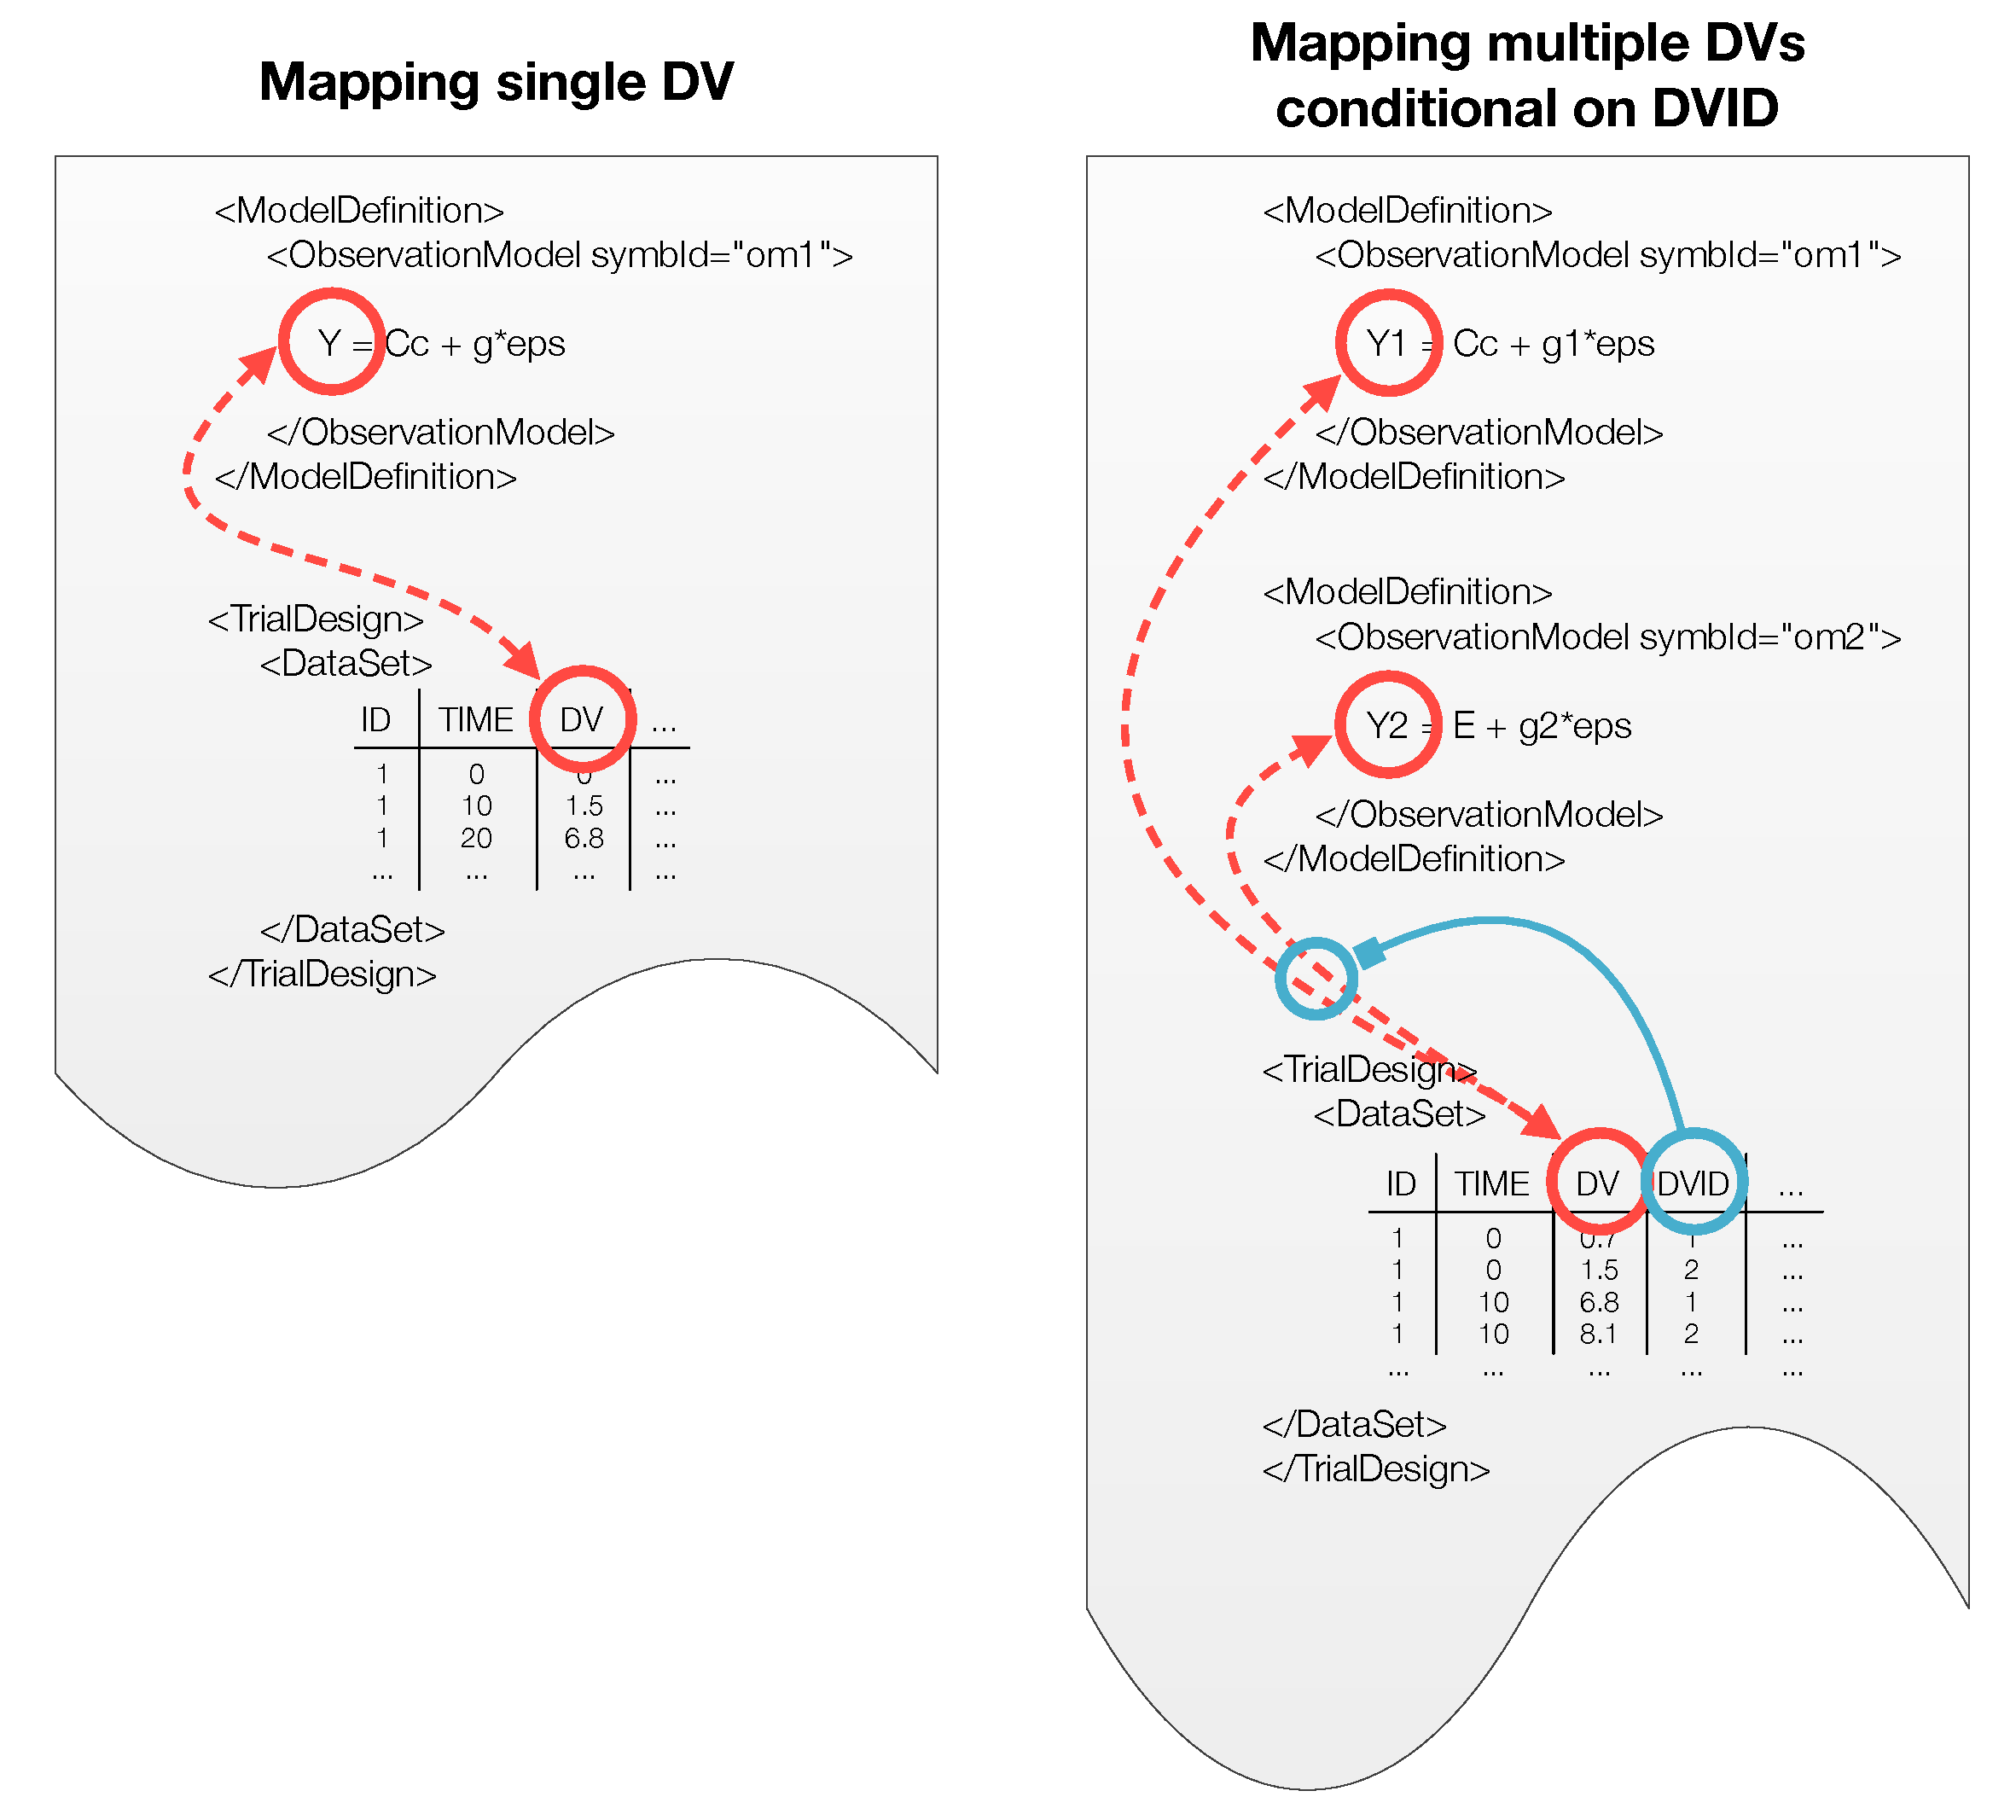
\includegraphics[width=120mm]{pics/mapping1.pdf}
% \caption{....}
% \label{fig:mappingDV}
%\end{figure}


\section{Markov models}
\label{sec:markovModels}
Stimulated by the discussion on the DDMoRE forum, a number of Markov models
was considered. The description and implementation details are given in the following 
sections. 

\subsection{Example 1 -- Simple Markov Model}
\label{subsec:exp1}

\subsection*{Model definition}
\subsubsection*{Observation model}

\begin{itemize}
\item
Type of observed variable -- discrete / categorical
\item
Category variable: $Y$
\item
Initial state variable: $Y_{init}$
\item
Set of categories: $\{\mbox{Alive}, \mbox{Dead}\}$
\item
Transition probability
\begin{align}
& P(\mbox{Alive} \rightarrow \mbox{Dead}) = 0.05 \nonumber
\end{align}
\end{itemize}

\subsection*{Trial Design}

\begin{itemize}
\item
Observations: Y at t=1,...,10.
\end{itemize}


\subsection*{Modelling steps}

\begin{itemize}
\item
Initial states
\begin{align}
& Y_{init} = \left( \begin{array}{c} 100 \\ 0 \end{array} \right) \nonumber
\end{align}
\end{itemize}


\subsection*{PharmML implementation}

\lstset{language=XML}
\begin{lstlisting}
    <ModelDefinition>
        <!-- OBSERVATIONS -->
        <ObservationModel blkId="om1">
            <Discrete>
                <CategoricalData>
                    
                    <ListOfCategories> 
                        <Category symbId="Alive"/>
                        <Category symbId="Dead"/>
                    </ListOfCategories>
                    
                    <CategoryVariable symbId="Y"/>

		    <!-- 100 people - see ModellingSteps/SimulationStep -->
                    <InitialStateVariable symbId="Yinit"/>
                    <PreviousStateVariable symbId="Yp"/>
                    
                    <Dependance type="discreteMarkov"/>
                    
                    <!-- P(Y=Dead|Yp=Alive)=0.05 -->
                    <ProbabilityAssignment>
                        <Probability symbId="p1">
                            <CurrentState>
                                <math:LogicBinop op="eq">
                                    <ct:SymbRef symbIdRef="Y"/>
                                    <ct:SymbRef symbIdRef="Dead"/>
                                </math:LogicBinop>
                            </CurrentState>
                            <PreviousState>
                                <math:LogicBinop op="eq">
                                    <ct:SymbRef symbIdRef="Yp"/>
                                    <ct:SymbRef symbIdRef="Alive"/>
                                </math:LogicBinop>
                            </PreviousState>
                        </Probability>
                        <ct:Assign>
                            <ct:Real>0.05</ct:Real>
                        </ct:Assign>
                    </ProbabilityAssignment>
                    
                </CategoricalData>
            </Discrete>
        </ObservationModel>
    </ModelDefinition>
\end{lstlisting}
Trial design: output of variable $Y$ at t=1,...,10.
\lstset{language=XML}
\begin{lstlisting}
    <TrialDesign>
        <Observations>
            <Observation oid="obsOid">
                <ObservationTimes>
                    <ct:Assign>
                        <ct:Sequence>
                            <ct:Begin><ct:Real>1</ct:Real></ct:Begin>
                            <ct:StepSize><ct:Real>1</ct:Real></ct:StepSize>
                            <ct:End><ct:Real>10</ct:Real></ct:End>
                        </ct:Sequence>
                    </ct:Assign>
                </ObservationTimes>
                <Discrete>
                    <ct:SymbRef blkIdRef="om1" symbIdRef="Y"/>
                </Discrete>
            </Observation>
        </Observations>
    </TrialDesign>
\end{lstlisting}
Modelling step definition and initial assignments, $Y_{init} = (100, 0)$
\lstset{language=XML}
\begin{lstlisting}
    <mstep:ModellingSteps>
        <mstep:SimulationStep oid="simOid">
            
            <mstep:ObservationsReference>
                <ct:OidRef oidRef="obsOid"/>
            </mstep:ObservationsReference>
            
            <ct:VariableAssignment>
                <ct:SymbRef blkIdRef="om1" symbIdRef="Yinit"/>
                <ct:Assign>
                    <ct:Vector>
                        <ct:VectorElements>
                            <ct:Real>100</ct:Real>
                            <ct:Real>0</ct:Real>
                        </ct:VectorElements>
                    </ct:Vector>
                </ct:Assign>
            </ct:VariableAssignment>
\end{lstlisting}



\subsection{Example 2 -- Three State Markov Model}
\label{subsec:exp2}

The next example is build around a Markov chain for three states/categories
which is shown in the figure \ref{fig:example2} and expressed by a set
of pair-wise transition probabilities or a so-called \textbf{left} transition 
(aka stochastic) matrix, on the right in the figure.
\begin{figure}[ht!]
\centering
  \includegraphics[width=120mm]{pics/example2.pdf}
 \caption{Example 2 can be expressed by the basic Markov chain with the
 transition probabilities given below or the transition matrix (right).}
 \label{fig:example2}
\end{figure}


\subsection*{Model definition}
\subsubsection*{Observation model}

\begin{itemize}
\item
Type of observed variable -- discrete / categorical
\item
Category variable: $Y$
\item
Initial state variable: $Y_{init}$
\item
Set of categories: $\{\mbox{Healthy}, \mbox{Sick}, \mbox{Dead}\}$
\item
Transition probabilities
\begin{itemize}
\item
as pairwise conditional transition probabilities
\begin{align}
& P(\mbox{Healthy} \rightarrow \mbox{Dead}) = 0.1 \nonumber \\
& P(\mbox{Healthy} \rightarrow \mbox{Sick}) = 0.2 \nonumber \\
& P(\mbox{Sick} \rightarrow \mbox{Healthy}) = 0.1 \nonumber \\
& P(\mbox{Sick} \rightarrow \mbox{Dead}) = 0.3 \nonumber
\end{align}
\item
or as transition (aka stochastic) matrix
%\[
%\begin{bmatrix}
%    1-0.2-0.1 & 0.2 & 0.01  \\
%    0.1 & 1-0.1-0.3 & 0.03  \\
%    0 & 0 & 1  \\
%\end{bmatrix}
%\]
\[
\begin{blockarray}{cccc}
& H & S & D \\
\begin{block}{c[ccc]}
H &    1-0.2-0.1 & 0.2 & 0.1  \\
S &    0.1 & 1-0.1-0.3 & 0.3  \\
D &    0 & 0 & 1  \\
\end{block}
\end{blockarray}
\]

\end{itemize}
\end{itemize}


\subsection*{Trial Design}

\begin{itemize}
\item
Observations: Y at t=1,...,10.
\end{itemize}


\subsection*{Modelling steps}

\begin{itemize}
\item
Initial states
\begin{align}
& Y_{init} = \left( \begin{array}{c} 100 \\ 0 \\ 0 \end{array} \right) \nonumber
\end{align}
\end{itemize}



\subsection*{PharmML implementation}
The model is a straightforward extension of example 1 for three categories and should
not be shown here except the transition matrix which can be used instead of
the transition probabilities 
\lstset{language=XML}
\begin{lstlisting}
<TransitionMatrix>
    <ct:Matrix matrixType="Any">
        <ct:ColumnNames>
            <ct:SymbRef symbIdRef="Healthy"/>
            <ct:SymbRef symbIdRef="Sick"/>
            <ct:SymbRef symbIdRef="Dead"/>
        </ct:ColumnNames>
        <ct:MatrixRow>
            <ct:Real>0.7</ct:Real><ct:Real>0.2</ct:Real><ct:Real>0.1</ct:Real>
        </ct:MatrixRow>
        <ct:MatrixRow>
            <ct:Real>0.1</ct:Real><ct:Real>0.6</ct:Real><ct:Real>0.3</ct:Real>
        </ct:MatrixRow>
        <ct:MatrixRow>
            <ct:Real>0</ct:Real><ct:Real>0</ct:Real><ct:Real>0.1</ct:Real>
        </ct:MatrixRow>
    </ct:Matrix>
</TransitionMatrix>
\end{lstlisting}


\subsection{Example 3 -- Stratified Markov Model}
\label{subsec:exp3}

The transition probabilities vary now conditional on the sex of 
the subjects. For example the probability for a healthy female to 
get sick is lower, 0.1, then for a male, 0.2. See Figure \ref{fig:markovMatrixCond}
for the Markov chain network and transition matrix for this model.

\begin{figure}[ht!]
\centering
  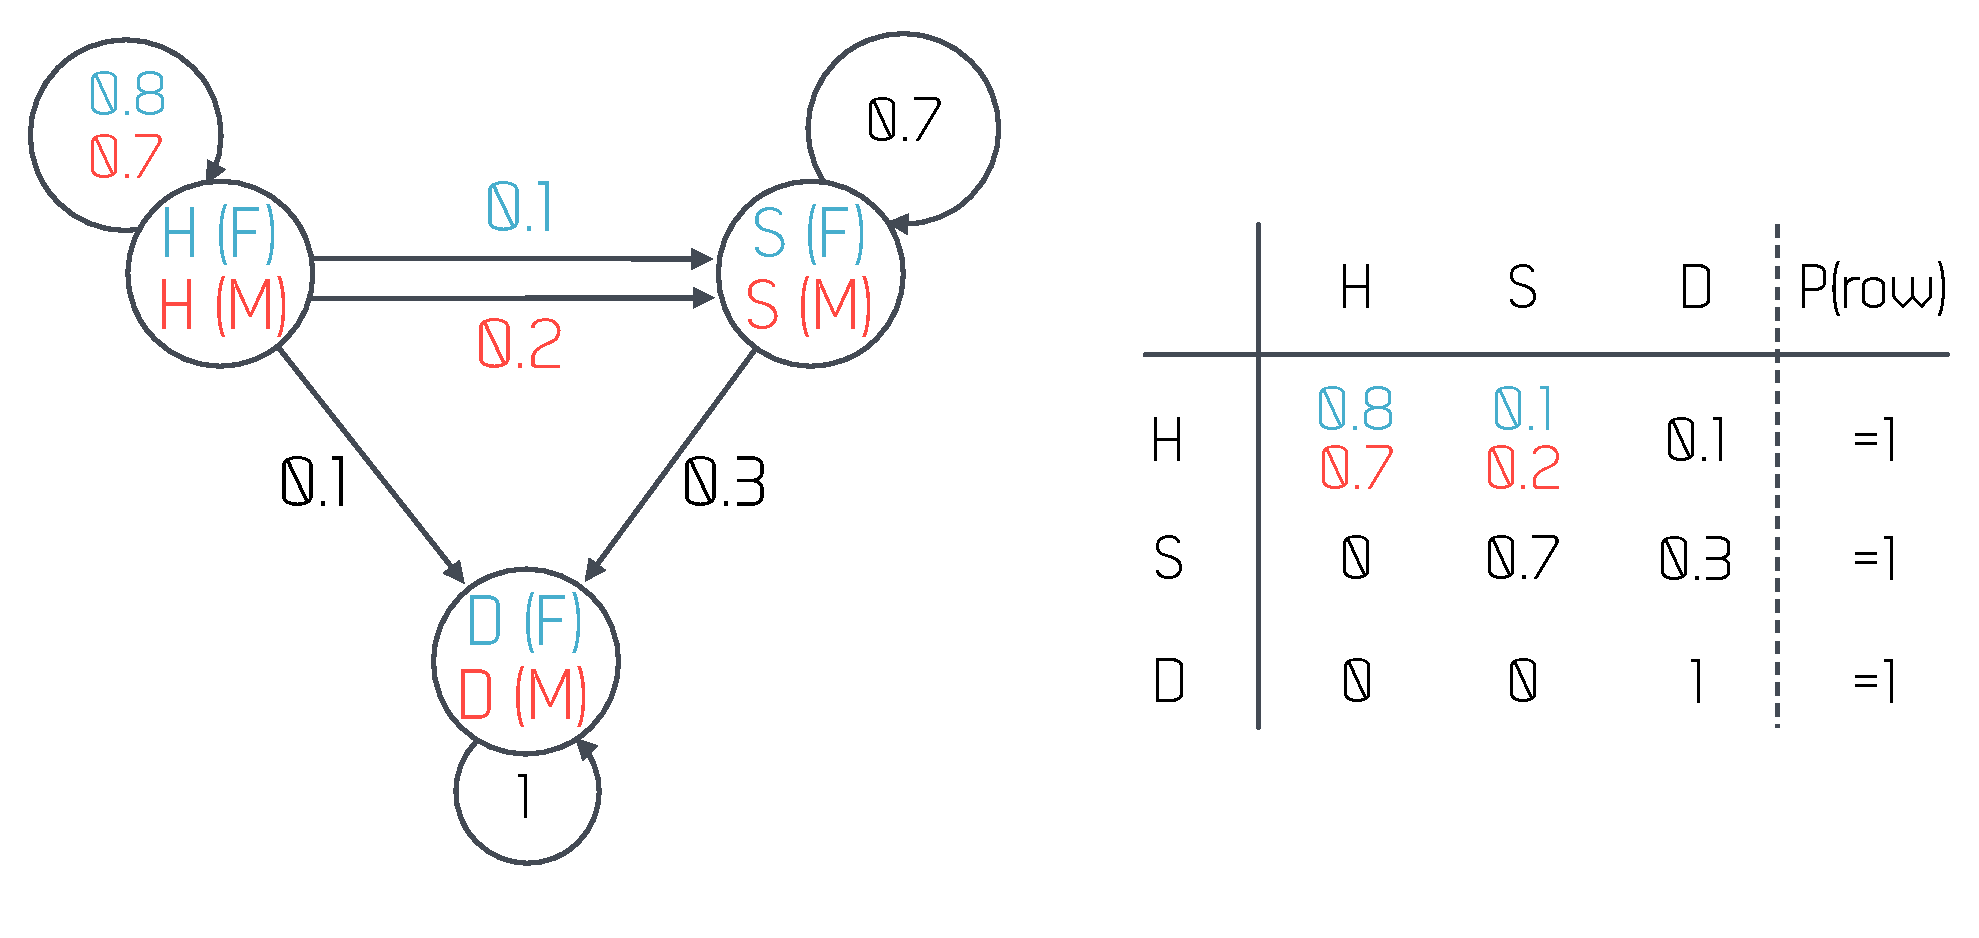
\includegraphics[width=120mm]{pics/markovMatrixCond.pdf}
 \caption{Example 3 -- a transition matrix defined conditional on sex of the subjects.}
 \label{fig:markovMatrixCond}
\end{figure}

\subsection*{Model definition}

\subsubsection*{Covariate model}
\begin{itemize}
\item
Age -- continuous covariate
\item
Sex = \{F, M\} -- categorical covariate
\end{itemize}

\subsubsection*{Observation model}

\begin{itemize}
\item
Type of observed variable -- discrete / categorical
\item
Category variable: $Y$
\item
Initial state variable: $Y_{init}$
\item
Set of categories: $\{\mbox{Healthy}, \mbox{Sick}, \mbox{Dead}\}$
\item
Transition probabilities
\begin{itemize}
\item
as pairwise conditional transition probabilities
\begin{align}
& P(\mbox{Healthy} \rightarrow \mbox{Sick} | \; SEX==F) = 0.1 \nonumber \\
& P(\mbox{Healthy} \rightarrow \mbox{Sick} | \; SEX==M) = 0.2 \nonumber \\
& P(\mbox{Sick} \rightarrow \mbox{Healthy}) = 0.1 \nonumber \\
& P(\mbox{Sick} \rightarrow \mbox{Dead}) = 0.3 \nonumber \\
& \mbox{other probabilities follow from the property 'left stochastic matrix'} \nonumber
\end{align}
\item
or as transition (aka stochastic) matrix
\[
\begin{blockarray}{cccc}
& H & S & D \\
\begin{block}{c[ccc]}
H &	0.7 & \left\{\begin{array}{ll}
      	0.1 & SEX== F \\
      	0.2 & SEX== M \\
\end{array}\right. & 0.1  \\\\
S &    0.1 & 0.6 & 0.3  \\\\
D &    0 & 0 & 1  \\
\end{block}
\end{blockarray}
\]
\end{itemize}
\end{itemize}

\subsection*{Trial Design}

\begin{itemize}
\item
Observations: Y at t=1,...,10.
\end{itemize}

\subsection*{Modelling steps}

\begin{itemize}
\item
Initial states
\begin{align}
& Y_{init} = \left( \begin{array}{c} 100 \\ 0 \\ 0 \end{array} \right) \nonumber
\end{align}
\end{itemize}

\subsection*{PharmML implementation}
Most of the model elements is identical to that of example in section \ref{subsec:exp2}
except the conditional transition probabilities, which XML encoding will be shown
here only.  The probabilities can be expresses pairwise or a transition matrix as the following 
code snippet show.

\begin{itemize}
\item
Pairwise probabilities (only the conditional ones are shown for brevity)

\lstset{language=XML}
\begin{lstlisting}
        <!-- P(Yp=Healthy -> Y=Sick | SEX=F)=0.1 -->
        <ProbabilityAssignment>
            <Probability>
                <CurrentState>
                    <math:LogicBinop op="eq">
                        <ct:SymbRef symbIdRef="Y"/>
                        <ct:SymbRef symbIdRef="Dead"/>
                    </math:LogicBinop>
                </CurrentState>
                <PreviousState>
                    <math:LogicBinop op="eq">
                        <ct:SymbRef symbIdRef="Yp"/>
                        <ct:SymbRef symbIdRef="Sick"/>
                    </math:LogicBinop>
                </PreviousState>
                <Condition>
                    <math:LogicBinop op="eq">
                        <ct:SymbRef symbIdRef="SEX"/>
                        <ct:CatRef catIdRef="F"/>
                    </math:LogicBinop>
                </Condition>
            </Probability>
            <ct:Assign>
                <ct:Real>0.1</ct:Real>
            </ct:Assign>
        </ProbabilityAssignment>
        
        <!-- P(Yp=Healthy -> Y=Sick | SEX=M)=0.1 -->
        <ProbabilityAssignment>
            <Probability>
                <CurrentState>
                    <math:LogicBinop op="eq">
                        <ct:SymbRef symbIdRef="Y"/>
                        <ct:SymbRef symbIdRef="Sick"/>
                    </math:LogicBinop>
                </CurrentState>
                <PreviousState>
                    <math:LogicBinop op="eq">
                        <ct:SymbRef symbIdRef="Yp"/>
                        <ct:SymbRef symbIdRef="Healthy"/>
                    </math:LogicBinop>
                </PreviousState>
                <Condition>
                    <math:LogicBinop op="eq">
                        <ct:SymbRef symbIdRef="SEX"/>
                        <ct:CatRef catIdRef="M"/>
                    </math:LogicBinop>
                </Condition>
            </Probability>
            <ct:Assign>
                <ct:Real>0.2</ct:Real>
            </ct:Assign>
        </ProbabilityAssignment>
\end{lstlisting}

\item
Transition matrix -- we use the fact that a matrix element can contain an arbitrary expression,
also a piecewise function used here for the transition probability from the \emph{Healthy} to 
\emph{Sick} state conditioned on the covariate \emph{Sex}. 
\lstset{language=XML}
\begin{lstlisting}
        <TransitionMatrix symbId="T1">
            <ct:Matrix matrixType="Any">
                <ct:ColumnNames>
                    <ct:SymbRef symbIdRef="Healthy"/>
                    <ct:SymbRef symbIdRef="Sick"/>
                    <ct:SymbRef symbIdRef="Dead"/>
                </ct:ColumnNames>
                <ct:MatrixRow>
                    <ct:Real>0.7</ct:Real>
                    <ct:Assign>
                        <ct:Piecewise>
                            <math:Piece>
                                <ct:Real>0.8</ct:Real>
                                <math:Condition>
                                    <math:LogicBinop op="eq">
                                        <ct:SymbRef symbIdRef="Sex"/>
                                        <ct:CatRef catIdRef="F"/>
                                    </math:LogicBinop>
                                </math:Condition>
                            </math:Piece>
                            <math:Piece>
                                <ct:Real>0.7</ct:Real>
                                <math:Condition>
                                    <math:LogicBinop op="eq">
                                        <ct:SymbRef symbIdRef="Sex"/>
                                        <ct:CatRef catIdRef="M"/>
                                    </math:LogicBinop>
                                </math:Condition>
                            </math:Piece>
                        </ct:Piecewise>
                    </ct:Assign>
                    <ct:Real>0.1</ct:Real>
                </ct:MatrixRow>
                <ct:MatrixRow>
                    <ct:Real>0.1</ct:Real><ct:Real>0.6</ct:Real><ct:Real>0.3</ct:Real>
                </ct:MatrixRow>
                <ct:MatrixRow>
                    <ct:Real>0</ct:Real><ct:Real>0</ct:Real><ct:Real>0.1</ct:Real>
                </ct:MatrixRow>
            </ct:Matrix>
        </TransitionMatrix>
\end{lstlisting}
\end{itemize}
Note, that the order of probabilities is defined by the order of categories/states names in the \xelem{ColumnNames}.
Because the transition matrix is symmetric specifying only the column names is sufficient. 

\subsection{Example 4 -- Micro Simulation Model}
\label{subsec:exp4}

\subsection*{Model definition}

\subsubsection*{Covariate model}
\begin{itemize}
\item
Age -- continuous covariate
\item
Sex = \{F, M\} -- categorical covariate
\end{itemize}
Individual covariates are stored in the trial design, see below.

\subsubsection*{Observation model}

\begin{itemize}
\item
Type of observed variable -- discrete / categorical
\item
Category variable: $Y$
\item
Initial state variable: $Y_{init}$
\item
Set of categories: $\{\mbox{Healthy}, \mbox{Sick}, \mbox{Dead}\}$
\item
Transition probabilities
\begin{itemize}
\item
as pairwise conditional transition probabilities
%
%Healthy to Dead: Age/1000\\
%Healthy to Sick: 0.1* (1 + Male) + 0.01*Age and never more than 0.8\\
%Sick to Healthy 0.1\\
%Sick to Dead:  0.01*Age+0.2*Male and never more than 0.9
\begin{align}
& P(\mbox{Healthy} \rightarrow \mbox{Dead}) = \mbox{Age}/100 \nonumber \\
p_{HS} := \quad & P(\mbox{Healthy} \rightarrow \mbox{Sick} | \; p_{HS} < 0.8) = 0.1(1 + \mbox{Male}) + 0.01\times\mbox{Age} \nonumber \\
& P(\mbox{Sick} \rightarrow \mbox{Healthy}) = 0.1 \nonumber \\
p_{SD} := \quad & P(\mbox{Sick} \rightarrow \mbox{Dead} | \; p_{SD} < 0.9) = 0.01\times\mbox{Age}+0.2\times\mbox{Male} \nonumber
\end{align}
\item
Transition matrix becomes complex with the additional boundaries
on the probabilities and it's probably a better to encode it pairwise
as above.
%\[
%T1 = 
%\begin{blockarray}{cccc}
%& \mbox{H} & \mbox{S} & \mbox{D} \\
%\begin{block}{c[ccc]}
%\mbox{H} & 0.7 	& 0.1(1 + \mbox{Male}) + 0.01\times\mbox{Age } \& \;p_{HS} < 0.8 & 0.1  \\\\
%\mbox{S} 	& 0.1 	& 0.6 & 0.01\times\mbox{Age}+0.2\times\mbox{Male } \& \;p_{SD} < 0.9  \\\\
%\mbox{D} 	& 0 		& 0 & 1  \\
%\end{block}
%\end{blockarray}
%%
%%\begin{bmatrix}
%%    0.7 & 0.2 & 0.01  \\
%%    0.1 & 0.6 & 0.03  \\
%%    0 & 0 & 1  \\
%%\end{bmatrix}
%\]
\end{itemize}
\end{itemize}



\subsection*{Trial Design}

\begin{itemize}
\item
Observations: Y at t=1,...,10.
\item
Covariates
\begin{itemize}
\item
continuous: Age = 1, 2, 3, 4, ..., 100

\item
categorical: Sex = \{F, M\} with Male = 0,1,0,1 .... (100 times)
\end{itemize}
\end{itemize}



\subsection*{Modelling steps}

\begin{itemize}
\item
Initial states
\begin{align}
& Y_{init} = \left( \begin{array}{c} 100 \\ 0 \\ 0 \end{array} \right) \nonumber
\end{align}
\end{itemize}

\subsection*{PharmML implementation}
The covariates are coming here as individual values, meaning that they
have to be provided as a table. This is when the \xelem{TrialDesign} is
very helpful as it is equipped with the required structure.
It is sufficient to declare the covariates in the \xelem{CovariateModel} within 
\xelem{ModelDefinition} as the following snippet shows
\lstset{language=XML}
\begin{lstlisting}
        <CovariateModel blkId="cm1">
            <Covariate symbId="AGE">
                <Continuous/>
            </Covariate>
            
            <Covariate symbId="MALE">
                <Categorical>
                    <Category catId="F"/>
                    <Category catId="M"/>
                </Categorical>
            </Covariate>
        </CovariateModel>
\end{lstlisting}
the proper values are stored then in the \xelem{IndividualCovariates} in 
\xelem{TrialDesign}
\lstset{language=XML}
\begin{lstlisting}
        <Covariates>
            <!--    Male = 0,1,0,1 .... (100 times)
                    Age = 1,2,3,4,...100-->
            <IndividualCovariates>
                <ColumnMapping>
                    <ds:ColumnRef columnIdRef="SEX"/>
                    <ct:SymbRef blkIdRef="cm1" symbIdRef="Sex"/>
                    <ds:CategoryMapping>
                        <ds:Map dataSymbol="1" modelSymbol="F"/>
                        <ds:Map dataSymbol="0" modelSymbol="M"/>
                    </ds:CategoryMapping>
                </ColumnMapping>
                <ColumnMapping>
                    <ds:ColumnRef columnIdRef="AGE"/>
                    <ct:SymbRef blkIdRef="cm1" symbIdRef="Age"/>
                </ColumnMapping>
                <ds:DataSet>
                    <ds:Definition>
                        <ds:Column columnId="ID" columnType="id" valueType="id" columnNum="1"/>
                        <ds:Column columnId="SEX" columnType="covariate" valueType="real" columnNum="2"/>
                        <ds:Column columnId="AGE" columnType="covariate" valueType="real" columnNum="3"/>
                    </ds:Definition>
                    <ds:Table>
                        <ds:Row>
                            <ct:Id>i1</ct:Id><ct:Real>0</ct:Real><ct:Real>1</ct:Real>
                        </ds:Row>
                        <ds:Row>
                            <ct:Id>i1</ct:Id><ct:Real>1</ct:Real><ct:Real>2</ct:Real>
                        </ds:Row>
                        <ds:Row>
                            <ct:Id>i1</ct:Id><ct:Real>0</ct:Real><ct:Real>3</ct:Real>
                        </ds:Row>
                        <ds:Row>
                            <ct:Id>i1</ct:Id><ct:Real>1</ct:Real><ct:Real>4</ct:Real>
                        </ds:Row>
                        <!-- omitted subjects -->
                        <ds:Row>
                            <ct:Id>i100</ct:Id><ct:Real>1</ct:Real><ct:Real>100</ct:Real>
                        </ds:Row>
                    </ds:Table>
                </ds:DataSet>
            </IndividualCovariates>
        </Covariates>
    </TrialDesign>
\end{lstlisting}
\xelem{ColumnMapping} elements are declared to provide the required information 
how to connect the model and the covariates.

From the model definition we show here only the implementation of one
probability, $P(\mbox{Sick} \rightarrow \mbox{Dead} | \; p_{SD} < 0.9)$, the remaining transition 
probabilities are analog.
\lstset{language=XML}
\begin{lstlisting}
        <!-- Healthy to Sick -->
        <!-- pHS:= P(y=Dead|yp=Healthy & pHS<0.8 = 0.1* (1 + Male) +  0.01*Age -->
        <ProbabilityAssignment>
            <Probability symbId="pHS">
                <CurrentState>
                    <math:LogicBinop op="eq">
                        <ct:SymbRef symbIdRef="y"/>
                        <ct:SymbRef symbIdRef="Sick"/>
                    </math:LogicBinop>
                </CurrentState>
                <PreviousState>
                    <math:LogicBinop op="eq">
                        <ct:SymbRef symbIdRef="yp"/>
                        <ct:SymbRef symbIdRef="Healthy"/>
                    </math:LogicBinop>
                </PreviousState>
                <Condition>
                    <math:LogicBinop op="lt">
                        <ct:SymbRef symbIdRef="pHS"/>
                        <ct:Real>0.8</ct:Real>
                    </math:LogicBinop>
                </Condition>
            </Probability>
            <ct:Assign>
                <math:Binop op="plus">
                    <math:Binop op="times">
                        <ct:Real>0.1</ct:Real>
                        <math:Binop op="plus">
                            <ct:Real>1</ct:Real>
                            <ct:SymbRef symbIdRef="Male"/>
                        </math:Binop>
                    </math:Binop>
                    <math:Binop op="times">
                        <ct:Real>0.01</ct:Real>
                        <ct:SymbRef symbIdRef="Age"/>
                    </math:Binop>
                </math:Binop>
            </ct:Assign>
        </ProbabilityAssignment>
\end{lstlisting}
Note, that the probability is assigned a symbol identifier \xatt{symbId="pHS"}
which is then used to express the condition $p\_{SD}<0.9$

\subsection*{Out of scope}
Compared to the original description there are model elements which 
definition will differ between the proposed models formulation and their  
PharmML implementation such as
\begin{itemize}
\item 
Definition of the simulation execution, here from the original description: \emph{ [...] each time 
step we want Age of each individual to increase by 1 before any transitions 
are executed: Age $\leftarrow$ Age + 1: This is executed for living individuals only}

Although it is not possible to define such simulation steps explicitly, it
is possible to encode them implicitly using covariate/regressors via lookup 
tables or other elements available in the \xelem{TrialDesign}. 
\item 
Output definition, here from the original description: \emph{[...] number of people in each 
state each year total and stratified by age groups above and below 50, and Male.} \\
Such analysis is assumed to be carried out by a downstream tool as it was 
not in the scope and requirements for PharmML.
\end{itemize}


%\section{Multiple infusions}
%
%Alternatively, you could use DesignParameter to encode the 
%amount vector
%\lstset{language=XML}
%\begin{lstlisting}
%		<mdef:DesignParameter symbId="doseAmountVector">
%			<ct:Assign>
%				<ct:Vector>
%					<ct:VectorElements>
%						<ct:Real>1</ct:Real>
%						<ct:Real>2</ct:Real>
%						<ct:Real>1</ct:Real>
%						<ct:Real>5</ct:Real>
%						<!-- ... -->
%					</ct:VectorElements>
%				</ct:Vector>
%			</ct:Assign>
%		</mdef:DesignParameter>
%\end{lstlisting}
%
%and then refer to it in (see in bold below)
%\lstset{language=XML}
%\begin{lstlisting}
%	<Interventions>
%		<Administration oid="inf1">
%			<Infusion>
%				<DoseAmount>
%					<ct:SymbRef symbIdRef="Ad"/>
%					<ct:Assign>
%						<math:Binop op="divide">
%							<math:Binop op="times">
%								<ct:SymbRef symbIdRef="doseAmountVector"/>
%								<ct:SymbRef blkIdRef="mmcvt" symbIdRef="wgt" />
%							</math:Binop>
%							<ct:SymbRef blkIdRef="mmpar" symbIdRef="V" />
%						</math:Binop>
%					</ct:Assign>
%				</DoseAmount>
%				<DosingTimes>
%					<ct:Assign>
%						<ct:Vector>
%							<ct:VectorElements>
%								<ct:Real>0</ct:Real>
%								<ct:Real>5</ct:Real>
%								<ct:Real>10</ct:Real>
%								<!-- ... -->
%							</ct:VectorElements>
%						</ct:Vector>
%					</ct:Assign>
%				</DosingTimes>
%				<Rate>
%					<ct:Assign>
%						<ct:Vector>
%							<ct:VectorElements>
%								<ct:Real>10</ct:Real>
%								<ct:Real>15</ct:Real>
%								<ct:Real>20</ct:Real>
%								<!-- ... -->
%							</ct:VectorElements>
%						</ct:Vector>	
%					</ct:Assign>
%				</Rate>
%				ALTERNATIVE 
%				<Duration>
%					<ct:Assign>
%						<ct:Vector>
%							<ct:VectorElements>
%								<ct:Real>10</ct:Real>
%								<ct:Real>15</ct:Real>
%								<ct:Real>20</ct:Real>
%								<!-- ... -->
%							</ct:VectorElements>
%						</ct:Vector>
%					</ct:Assign>
%				</Duration>
%			</Infusion>
%		</Administration>
%\end{lstlisting}
%















